\section{TOKIO Architecture \& Implementation} \label{sec:architecture}

\begin{figure}[t]
    \centering
    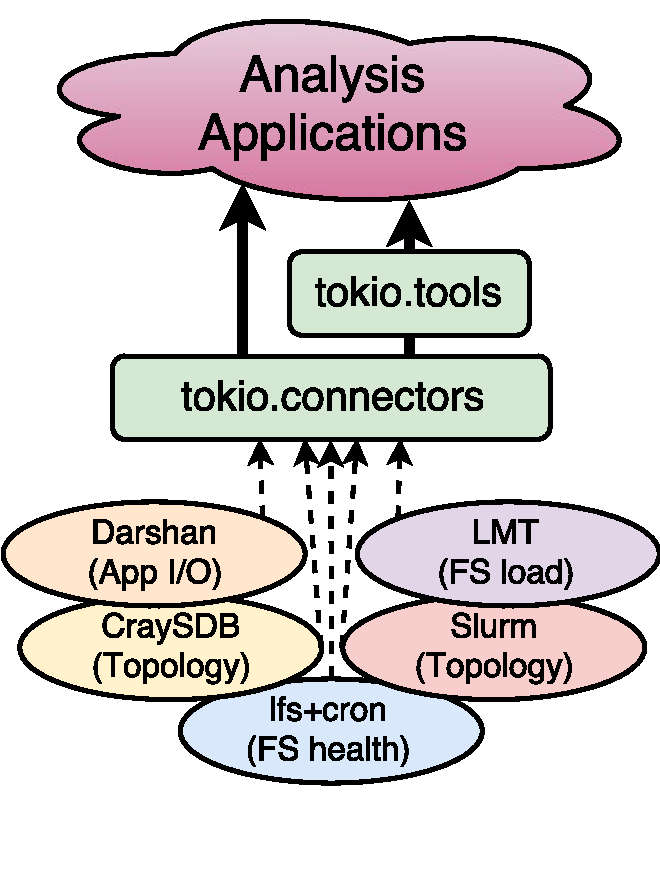
\includegraphics[width=0.7\columnwidth]{tokio-architecture-v3}
    \vspace{-.3in}
    \caption{TOKIO Architecture.  \texttt{tokio.connectors} take input from component-level monitoring tools in their native output formats and expose that data to upstream analysis in standard data formats such as key-value pairs, Pandas dataframes, and NumPy arrays. \texttt{tokio.tools} provide indices, site-specific data placement information, and enhanced usability.}
    \label{fig:tokio-architecture}
    \vspace{-.2in}
\end{figure}

\TODO{Describe a high-level overview of TOKIO here.  Design motivations = do everything as unprivileged user.}

The TOKIO framework is comprised of four layers as shown in Figure \ref{fig:tokio-architecture}.  By connecting many of the components included with Cray systems, pytokio enables a holistic view of I/O performance and file system health without the need to provision new monitoring infrastructure.

\subsection{Component-level monitoring tools} \label{sec:architecture/components}

are the I/O profiling and monitoring tools that are already used by HPC centers to profile application I/O patterns (e.g., Darshan~\cite{Carns2009}) and monitor file system server loads (e.g., LMT~\cite{Keopp2014} or Caribou~\cite{Flaskerud2017}), job topology (e.g., Cray's Service Database and Slurm), file system health (e.g., Lustre's \texttt{lfs df} and \texttt{lctl dl} commands), and other I/O components.

\subsection{TOKIO connectors} \label{sec:architecture/connectors}

interact with component-level tools using each tool's native interface and data formats and translate these tool-specific formats into semantically consistent data objects.  In the pytokio implementation of TOKIO, connectors are classes that expose each component-level tool's data as dictionaries, dataframes, and arrays.

pytokio provides connectors for the following tools either available as community-supported open-source tools or pre-installed on Cray systems:

\begin{itemize}
\item \textbf{Cray SDB} for node topology
\item \textbf{Slurm} for job ID and node list mappings
\item \textbf{Darshan} for application-level I/O profiling
\item \textbf{Lustre} \texttt{lfs} and \texttt{lctl} for file system health
\item \textbf{LMT} for server-side Lustre loads via the ClusterStor Lustre monitoring tool~\cite{Keopp2014}
\end{itemize}

\subsection{TOKIO tools} \label{sec:architecture/tools}

provide convenience functions and wrappers around TOKIO connectors.  For example, TOKIO provides a \texttt{topology} tool which converts a user job ID into a job radius by converting the job ID into a node list using the Slurm connector, and then the node list into topological coordinates using the Cray SDB connector.

\subsection{Analysis applications} \label{sec:architecture/analysis}

perform statistical, analytical, and visual performance analyses by using TOKIO connectors and tools to combine data from multiple components.